\documentclass{article}
\usepackage{graphicx}
\usepackage{amsmath}
\usepackage{hyperref}
\usepackage[margin=1in]{geometry}
\usepackage{booktabs} 
\title{Highly Efficient Geometric Brownian Motion Modeling with QMCPy}
\author{Larysa Matiukha and Sou-Cheng Choi}
\date{\today}
\begin{document}
\maketitle

\section{Introduction}

In this blog post, we demonstrate how to simulate and analyze a Geometric Brownian Motion (GBM) process using QMCPy in Python.
GBM is widely used in finance to model stock prices and other assets. 
We will walk through key code snippets, plots, and insights.

GBM is a continuous stochastic process in which the natural logarithm of its values follows a Brownian motion $[1]$.
Mathematically, it can be defined as follows:
$$\large{S_t = S_0 \, e^{\big(\mu - \frac{\sigma^2}{2}\big)  t + \sigma W_t}}, \label{gbm}$$
where
\begin{itemize}
\item $S_0$ is the initial value, 
\item $\mu$ is a drift coefficient
\item  $\sigma$ is difussion coefficient  
\item  $W_t$ is a (standard) Brownian motion.
\end{itemize}

At any time $t > 0$, $S_t$ follows a log-normal distribution with expected value and variance as follows (see Section 3.2 in $[1]$):
\begin{itemize}
\item
 $E[S_t] = S_0 e^{\mu t}$
\item $\text{Var}[S_t] = S_0^2 e^{2\mu t}(e^{\sigma^2 t} - 1)$
\item   $  
    \text{Cov}(S(t_i), S(t_j)) = S_0^2 e^{\mu(t_i + t_j)} \left(e^{\sigma^2 \min(t_i, t_j)} - 1\right).$
\end{itemize}


GBM is commonly used to model stock prices and options payoffs. 

\section{GBM object in QMCPy}

BBM in QMCPy inherits from BrownianMotion class $[2, 3]$. 
We can create a simple GBM instance and generate sample paths to see the class in action:
\begin{verbatim}
import qmcpy as qp
gbm = qp.GeometricBrownianMotion(qp.Lattice(2)) 
gbm.gen_samples(n=4) # generates four 2-dimensional samples
\end{verbatim}

Let's validate the  theoretical properties by generating a large number of GBM samples and comparing the empirical moments with the theoretical values. Note that the theoretical values match the last values captured in \texttt{qp\_gbm.mean\_gbm} and \texttt{qp\_gbm.covariance\_gbm} for the final time point. The results are reported in Table~\ref{tab1}.

\begin{verbatim}
# Generate GBM samples for theoretical validation
S0, mu, sigma, T, n_samples = 100.0, 0.05, 0.20, 1.0, 2**12
sampler = qp.Lattice(5, seed=42)
qp_gbm = qp.GeometricBrownianMotion(sampler, t_final=T, initial_value=S0, drift=mu, 
                                    diffusion=sigma)
paths = qp_gbm.gen_samples(n_samples)
S_T = paths[:, -1]  # Final values only

# Calculate theoretical vs empirical sample moments
theo_mean = S0 * np.exp(mu * T)
theo_var = S0**2 * np.exp(2*mu*T) * (np.exp(sigma**2 * T) - 1)
qp_emp_mean = np.mean(S_T)
qp_emp_var = np.var(S_T, ddof=1) 
\end{verbatim}

\begin{table}[t]
\centering
\caption{Theoretical vs Empirical Validation of GBM Properties}
\begin{tabular}{ll}
\hline
\textbf{Statistic} & \textbf{Value} \\
\hline
Sample Mean & 105.134 (Theoretical: 105.127) \\
Sample Variance & 453.062 (Theoretical: 451.029) \\
\hline
Time Vector & [0.2,\; 0.4,\; 0.6,\; 0.8,\; 1.0] \\
Drift ($\mu$) & 0.05 \\
Diffusion ($\sigma$) & 0.20\\
Mean  & [101.005,\; 102.020,\; 103.045,\; 104.081,\; 105.127] \\
Decomposition Type & PCA \\
\hline
\multicolumn{2}{l}{\textbf{Covariance Matrix:}} \\
\multicolumn{2}{l}{
\(
\begin{bmatrix}
81.943 & 82.767 & 83.599 & 84.439 & 85.288 \\
82.767 & 167.869 & 169.556 & 171.260 & 172.981 \\
83.599 & 169.556 & 257.923 & 260.516 & 263.134 \\
84.439 & 171.260 & 260.516 & 352.258 & 355.798 \\
85.288 & 172.981 & 263.134 & 355.798 & 451.029
\end{bmatrix}
\)
} \\
\hline
\end{tabular}
\label{tab1}
\end{table}


\section{GMB vs Brownian Motion}

Below we compare Brownian motion and geometric Brownian motion using the same parameters: $\texttt{drift} = 0$, $\texttt{diffusion} = 1$, $\texttt{initial\_value} = 1$.


First, let's define a utility function that will help us visualize GBM paths with different samplers and parameters:


\begin{verbatim}
def plot_paths(motion_type, sampler, t_final, initial_value, drift, diffusion, n):
    if motion_type.upper() == 'BM':
        motion = qp.BrownianMotion(sampler, t_final, initial_value, drift, diffusion)
        title = f'Realizations of Brownian Motion using {type(sampler).__name__} points'
        ylabel = 'W(t)'
    elif motion_type.upper() == 'GBM':
        motion = qp.GeometricBrownianMotion(sampler, t_final, initial_value, drift, diffusion)
        title = f'Realizations of Geometric Brownian Motion using {type(sampler).__name__} points'
        ylabel = 'S(t)'
    else:
        raise ValueError("motion_type must be 'BM' or 'GBM'")
    
    t = motion.gen_samples(n)
    initial_values = np.full((n, 1), motion.initial_value)
    t_w_init = np.hstack((initial_values, t))
    tvec_w_0 = np.hstack(([0], motion.time_vec))

    plt.figure(figsize=(7, 4));
    plt.plot(tvec_w_0, t_w_init.T); 
    plt.title(title);
    plt.xlabel('t');
    plt.ylabel(ylabel);
    plt.xlim([tvec_w_0[0], tvec_w_0[-1]]);
    plt.show();
\end{verbatim}


Paths of the driftless Brownian motion should fluctuate symmetrically around the initial value (y = 1) and can take negative values, while those of Geometric Brownian Motion remain strictly positive.

\begin{verbatim}
# Compare Brownian Motion and Geometric Brownian Motion using the unified plotting function
n = 16
sampler = qp.Lattice(2**7)
plot_paths('BM', sampler, t_final=1, initial_value=1, drift=0, diffusion=1, n=n)
plot_paths('GBM', sampler, t_final=1, initial_value=1, drift=0, diffusion=1, n=n)
\end{verbatim}

\begin{figure}[t!]
\centering
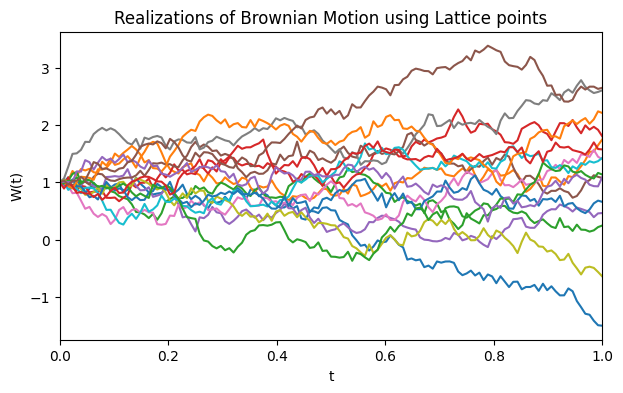
\includegraphics[width=0.49\textwidth]{images/figure_1.png}
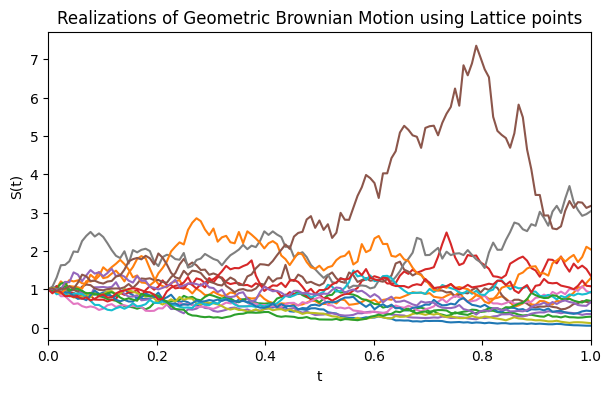
\includegraphics[width=0.49\textwidth]{images/figure_2.png}\\
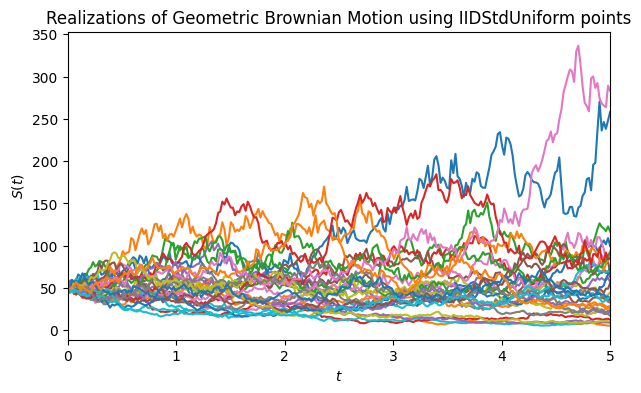
\includegraphics[width=0.49\textwidth]{images/figure_3.png}
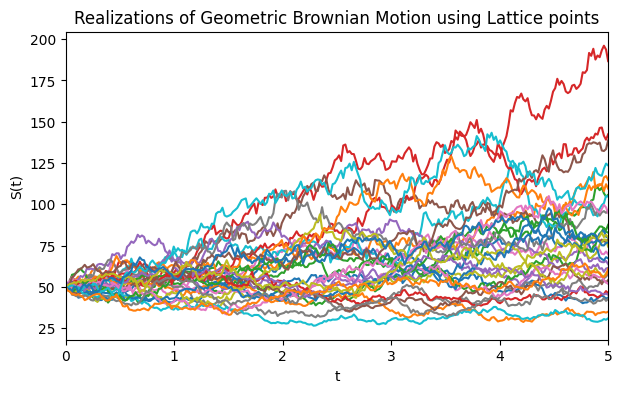
\includegraphics[width=0.49\textwidth]{images/figure_4.png}
\caption{Sample paths of BM and GBM.}
\end{figure}

Now, using \texttt{plot\_paths}, we generate 32 GBM paths to model stock price, $S(t)$, with initial value $S_0$ = 50, drift coeffient, $\mu = 0.1$, diffusion coefficient $\sigma = 0.2$ using IID points.


\begin{verbatim}
gbm_iid = plot_paths('GBM', qp.IIDStdUniform(2**8), t_final=5, 
                     initial_value=50, drift=0.1, diffusion=0.2, n=32)
\end{verbatim}



Using the same parameter values as in example above, we generate 32 GBM paths to model stock price using low-discrepancy lattice points:

\begin{verbatim}
gbm_lattice = plot_paths('GBM', qp.Lattice(2**8), t_final=5, 
                          initial_value=50, drift=0.1, diffusion=0.2, n=32)
\end{verbatim}



\section{QuantLib vs QMCPy Comparison}

In this section, we compare QMCPy's GeometricBrownianMotion implementation with the industry-standard QuantLib library [6] to validate its accuracy and performance. The numerical results are summarized in Table~\ref{tab2}.


\begin{verbatim}
import QuantLib as ql
import time

def generate_quantlib_paths(initial_value, mu, sigma, maturity, n_steps, n_paths):
    """Generate GBM paths using QuantLib"""
    process = ql.GeometricBrownianMotionProcess(initial_value, mu, sigma)
    rng = ql.GaussianRandomSequenceGenerator(ql.UniformRandomSequenceGenerator(n_steps, 
                                             ql.UniformRandomGenerator()))
    sequence_gen = ql.GaussianPathGenerator(process, maturity, n_steps, rng, False)
    start_time = time.time()
    paths = np.zeros((n_paths, n_steps + 1))
    for i in range(n_paths):
        sample_path = sequence_gen.next().value()
        paths[i, :] = np.array([sample_path[j] for j in range(n_steps + 1)])
    generation_time = time.time() - start_time
    return paths, generation_time

# Parameters
params = {'initial_value': 100, 'mu': 0.05, 'sigma': 0.2, 'maturity': 1.0, 'n_steps': 252, 
          'n_paths': 2**14}

# Generate paths 
quantlib_paths, quantlib_time = generate_quantlib_paths(**params)
\end{verbatim}


\begin{figure}[t!]
\centering
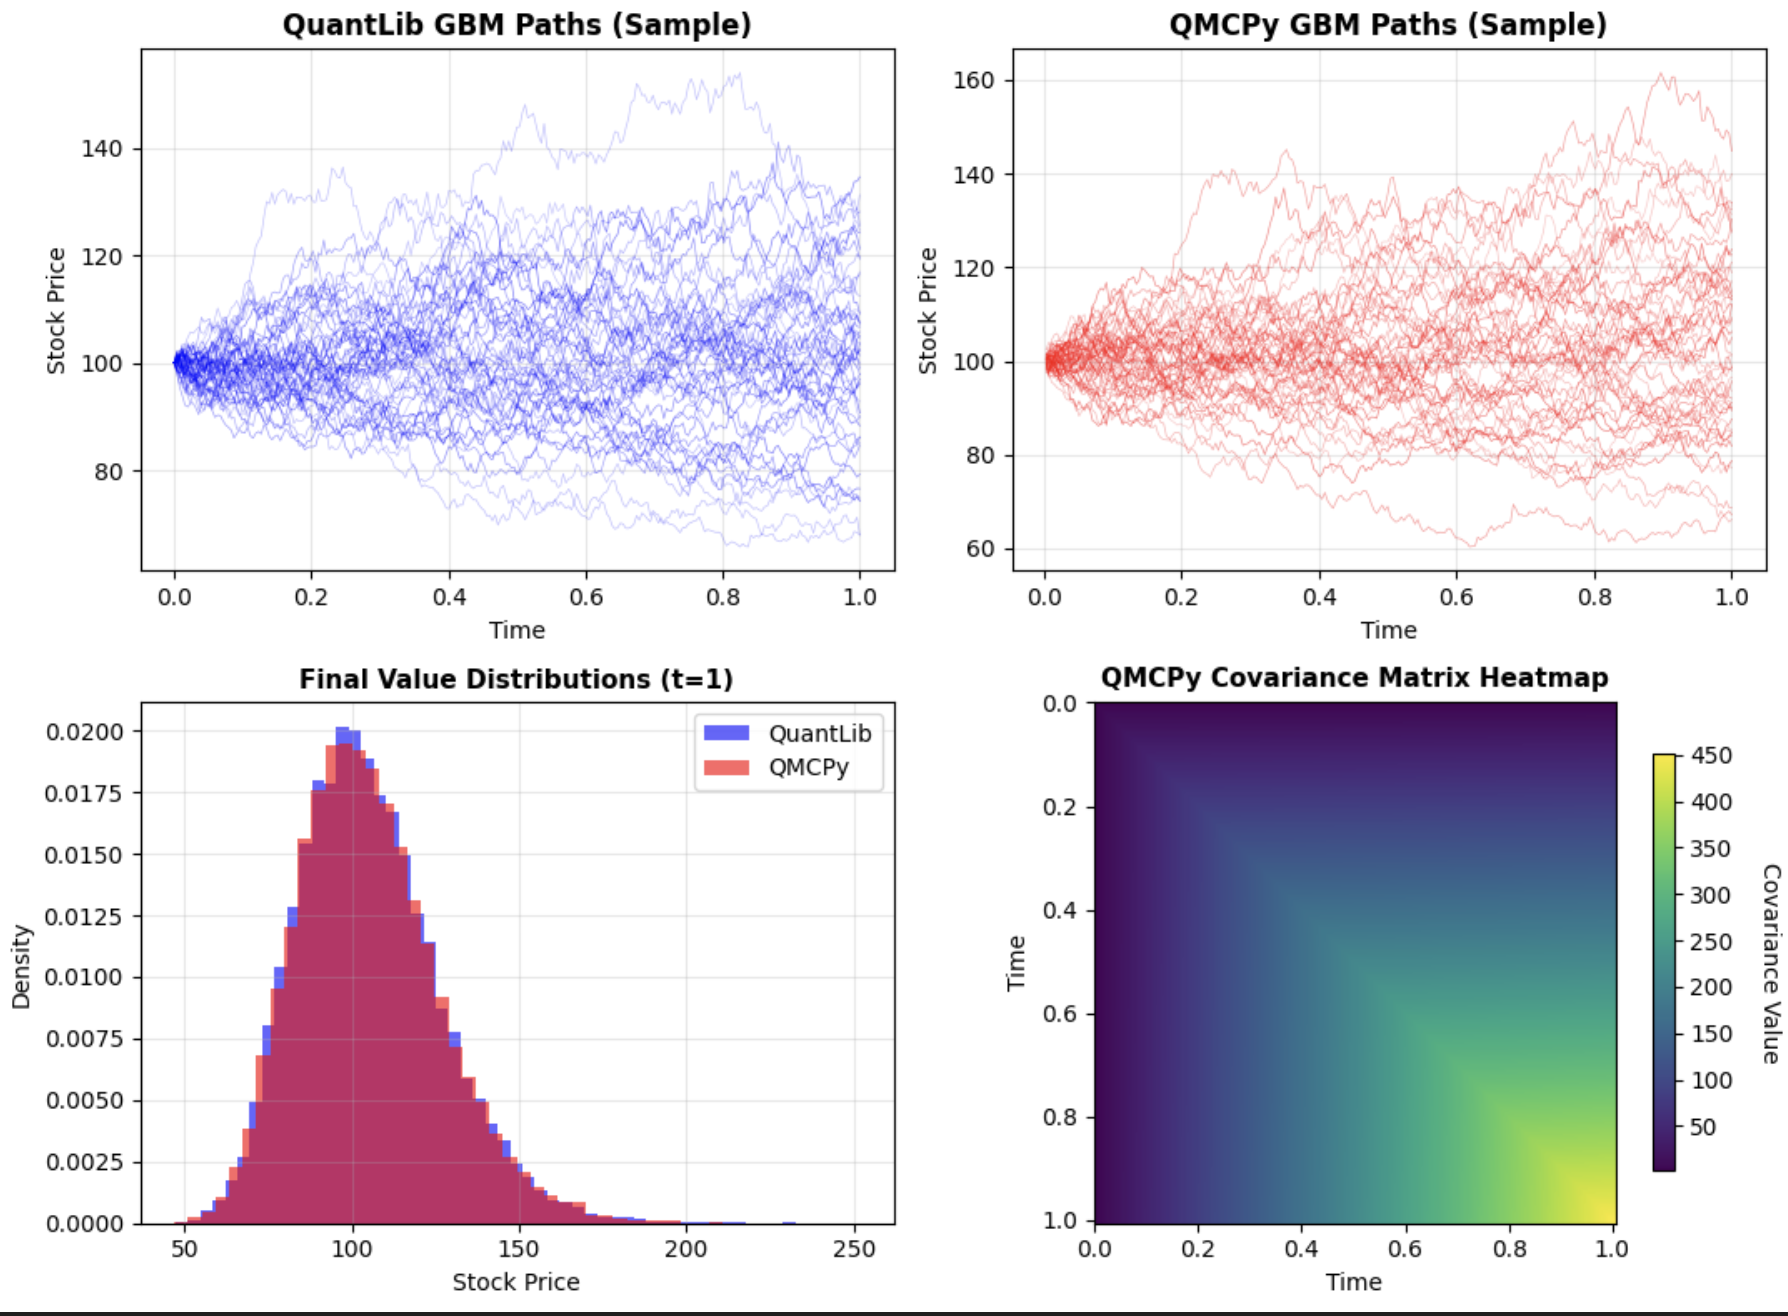
\includegraphics[width=1\textwidth]{images/figure_5.png}
\caption{QMCPy vs QuantLib: Both libraries produce statistically equivalent GBM simulations that match theoretical values. QMCPy typically runs 2-4 times faster due to vectorized operations, making it excellent for research and high-performance applications. QuantLib remains the industry standard for production systems requiring comprehensive  support for financial modeling and risk management.}
\end{figure}

\begin{table}[t]
\centering
\caption{QuantLib vs QMCPy: QMCPy is 3 times faster than QuantLib in generating thousands of paths.}
\begin{tabular}{lccc}
\toprule
\textbf{Method} & \textbf{Mean} & \textbf{Std. Dev.} & \textbf{Time (s)}   \\
\midrule
QuantLib & 105.10 & 21.11 & 0.817  \\
QMCPy & 105.13 & 21.25 & 0.270  \\
Theoretical & 105.13 & 21.24 & ---  \\
\bottomrule
\end{tabular}
\label{tab2}
\end{table}

\section{Internals}

The \texttt{GeometricBrownianMotion} class in QMCPy is engineered for speed, robustness, and mathematical correctness. Its design leverages object-oriented inheritance and vectorized operations, resulting in both flexibility and high performance.
\texttt{GeometricBrownianMotion} inherits from \texttt{BrownianMotion} which itself inherits from \texttt{Gaussian}. This layered design allows the GBM class to reuse and extend efficient implementations for Gaussian random vectors and Brownian motion increments.
The constructosr rigorously check input parameters (e.g., positivity of initial value and diffusion, valid decomposition type), ensuring mathematical integrity and preventing runtime errors.


The class uses vectorized NumPy operations to generate entire arrays of GBM paths in a single call, minimizing Python loops and maximizing computational throughput. Sample generation proceeds in two stages:
\begin{enumerate}
\item 
The parent class generates Brownian motion increments using the specified sampler (e.g., low-discrepancy lattice, IID uniform), with drift and diffusion handled in the mean and covariance structure.
\item  The GBM class transforms these increments via the exponential mapping    \eqref{gbm}, performed in a fully vectorized fashion, ensuring that thousands of paths can be simulated in milliseconds.
\end{enumerate}
The class computes and stores the theoretical mean and covariance matrices for GBM at initialization, which can be used for validation and theoretical comparisons. Both mean and covariance are calculated using analytical formulas, leveraging NumPy’s broadcasting for efficient computation.


The underlying Gaussian and Brownian motion classes support both Principal Component Analysis (PCA) and Cholesky decomposition for generating correlated increments. PCA is the default, offering better numerical stability and performance for high-dimensional simulations.

After path generation, the class can validate that all generated GBM values are strictly positive, as required by the mathematical definition. Violations raise errors or warnings, depending on strictness settings.
The \texttt{\_spawn} method allows for reproducible generation of new GBM instances with the same parameters but different samplers or dimensions, supporting advanced Monte Carlo workflows.  The design supports various samplers, including low-discrepancy sequences and IID random numbers, enabling both quasi-Monte Carlo and standard Monte Carlo simulations without code changes.
\section*{References}

\begin{enumerate}
\item  Paul Glasserman, P. (2003) *Monte Carlo Methods in Financial Engineering*. Springer, 2nd edition
\item  Choi, Sou-Cheng T.
and Hickernell, Fred J.
and Jagadeeswaran, Rathinavel
and McCourt, Michael J.
and Sorokin, Aleksei G. (2022) Quasi-Monte Carlo Software, In Alexander Keller, editor, *Monte Carlo and Quasi-Monte Carlo Methods* Springer International Publishing
\item S.-C. T. Choi and F. J. Hickernell and R. Jagadeeswaran and M. McCourt and A. Sorokin. (2023) QMCPy: A quasi-Monte Carlo Python Library (versions 1--1.6.2)
\item  Hull, J. C. (2017) *Options, Futures, and Other Derivatives*. Pearson, 10th edition
\item   Sheldon. Ross. (2014) *Introduction to Probability Models*. Academic Press, 11th edition
\item  QuantLib Development Team. QuantLib: A free/open-source library for quantitative finance, Version 1.38, https://www.quantlib.org
\end{enumerate}
 

\end{document}